\documentclass[a4paper]{beamer}
\usepackage[english]{babel}
\usepackage[utf8]{inputenc}
\usepackage{graphicx}
\usepackage{subcaption}
\usepackage{caption}
\usepackage{appendixnumberbeamer}
\usepackage{tikz}
\usepackage{csvsimple}
\usepackage{tabularx}
\usepackage{adjustbox}
\usepackage{pdfpages}
\usepackage{cleveref}
%\usepackage[orientation=paysage,size=A4]{beamerposter}
\usepackage{slashed}
\captionsetup{labelformat=empty,labelsep=none}
\beamertemplatenavigationsymbolsempty
\usetheme{Boadilla}

\title[Energy calibration \& Higgs couplings]{Calibration of the ATLAS electromagnetic calorimeter and measurement of the couplings of the (Brout-Englert-)Higgs boson in the diphoton channel}
\author[Goudet]{Christophe Goudet}
\institute[LAL]{\includegraphics[width=0.3\linewidth]{LAL.jpg} }

\date[Orsay, \today]{PhD defense \\ Orsay, \today}
\graphicspath{{/home/goudet/Documents/LAL/ExternalPlot/}{/home/goudet/Documents/LAL/Zim/Calibration/TemplateMethod/PlotsIllustration/}}

\newcommand{\tbfhyy}{\ensuremath{\times B(H \to \gamma\gamma)}}
\newcommand{\fb}{\ensuremath{\,\text{fb}}}
\def\pt{\ensuremath{p_{\rm T}}}


\begin{document}
\transboxin
\begin{frame}
\maketitle
\end{frame}

\begin{frame}{Introduction}
\tableofcontents
\end{frame}

\section{The Standard Model of matter}
%%=============================
\begin{frame}{Particle content of matter}
    Over the XX$^{th}$ century, elementary particles have been organised into a well structured model.

  \begin{center} \includegraphics[width=\linewidth]{OPEN-PHO-CHART-2015-001.png} \end{center}
\end{frame}
%% %%=============================
%% \begin{frame}{A mathematical framework}
%%   Matter knowledge is embedded into a well defined mathematical framework based on a Lagrangian $L$.

%%   \begin{equation}
%%     L = \frac{m \vec{\dot{q}}^2}{2} - V(\vec{q})
%%   \end{equation}

%%   The dirac lagrangian describes a massive fermion field :
%%   \begin{equation}
%%     L = \bar{\psi} ( i\slashed{\partial} - m ) \psi
%%   \end{equation}
  
%%   Imposing least action principle (similar to classical mechanic) lead to equations of motion :
%%   \begin{equation}
%%     \frac{\partial L}{\partial q} - \frac{d}{dt}\frac{\partial L}{\partial \dot{q}_i} = 0
%%   \end{equation}
  
%% \end{frame}
%% %%=============================
%% \begin{frame}{Gauge invariance}
%%   Symmetries are transformations which \textcolor{blue}{leave a system unchanged.}
%%   Imposing symmetries on a Lagrangian changes the theory it describes.
%%   \vfill
  
%%     \begin{equation}
%%       \psi(x)\rightarrow e^{i\alpha(x)}\psi(x)
%%     \end{equation}

%%     Derivative affects $e^{i\alpha}$\\
%%     $\rightarrow$ \textcolor{red}{\bf Invariance achieved by adding a field $A_\mu$ and changing $L$.} \\
%%     $\rightarrow$ mass term for $A$ ($m^2A_\mu A^\mu$) is forbidden by symmetries
%%     \begin{equation}
%%       \label{eq:orgc79752f}
%%       \partial_\mu\rightarrow D_\mu=\partial_\mu+ieA_\mu(x)
%%     \end{equation}
%%     \begin{equation}
%%       \label{eq:orge69917a}
%%       A_{\mu} \rightarrow A_\mu(x) - \frac{1}{e} {\partial_{\mu} \alpha(x)}
%%     \end{equation}


%%     \includegraphics[width=0.49\linewidth]{Iliopoulos_1f.pdf}
%%     \includegraphics[width=0.49\linewidth]{Iliopoulos_2f.pdf}


%% \end{frame}
%%=============================
\begin{frame}{Spontaneous Symmetry Breaking}
  SSB describes a system for which its ground state has less symmetry than its Lagrangian.

  \includegraphics[width=\linewidth]{SymBreakPen.jpg}
  \begin{itemize}
  \item Unstable equilibrium has cylindrical symmetry
  \item Ground state (fallen pen) ``has chosen'' a direction.
    The cylindrical symmetry has been broken.
  \end{itemize}
\end{frame}
%%=============================
\begin{frame}{SSB in field theory}
  SSB is created by imposing a ``mexican hat'' potential on a field.
  \begin{equation}
    \label{eq:orgdea495d}
    V(\phi) = \frac{1}{2}\mu^2\phi^*\phi+\frac{1}{4}\lambda(\phi^*\phi)^2
  \end{equation}
  with  $\lambda>0$ and $\mu^2 <0$.
  
  \begin{minipage}{0.49\linewidth}
  \begin{itemize}
  \item Potential has rotational symmetry
  \item Ground state $|\Phi|=\sqrt{-\frac{\mu^2}{2\lambda^2}}= \frac{\text{vev}}{\sqrt{2}}$ breaks symmetry.
  \item Describe a massless and a massive ($m^2=v^2\lambda$) bosons.
  \end{itemize}
  \end{minipage}
  \hfill
  \begin{minipage}{0.49\linewidth}
    \includegraphics[width=\linewidth]{MexicanHatPot.jpg}
  \end{minipage}
\end{frame}
%%=============================
\begin{frame}{The Standard Model}
  
  The SM is composed of :
  
  \begin{itemize}
  \item Local gauge symmetries
    \begin{itemize}
    \item $SU(3)_c$ for strong interaction. 8 gluons couple to quarks.
    \item $SU(2)_L\times U(1)_Y$ for electroweak sector. Bosons $W^\pm$, $Z$ and photon couple to quarks and leptons.
    \end{itemize}
    \vfill
  \item SSB of $SU(2)_L$ by introduction of scalar field $\Phi$
    \begin{itemize}
    \item gives mass to $W^\pm$ and $Z$.
    \item A physical and massive degree of freedom : the (Brout-Englert)-Higgs boson $H$.
    \item Yukawa coupling gives mass to fermions.
    \end{itemize}
  \end{itemize}
\end{frame}
%%=============================
\begin{frame}{Higgs boson production}
  $H$ boson predictions are function of its mass.
  
  \begin{minipage}{0.44\linewidth}
    \centering
    \includegraphics[width=\linewidth]{CERN-THESIS-2014-122_1f10.pdf}\\
    \includegraphics[width=\linewidth]{YRHXS_Summary_fig3.pdf}
  \end{minipage}
  \hfill
  \begin{minipage}{0.55\linewidth}
    4 dominant production modes
    \begin{itemize}
    \item Gluon fusion ($ggH\simeq 86\%$) probes coupling to gluons through loop.
    \item Vector Boson Fusion probes direct coupling to electroweak bosons.
    \item Higgsstrahlung also probes $W\pm$ and $Z$ couplings.
    \item Associated top production probes couplings to heaviest quark.
    \end{itemize}
  \end{minipage}
\end{frame}

%%=============================
\begin{frame}{Higgs boson decays}
  A Higgs boson with a mass around $125$~GeV opens a wide range of decay channels.
  
  \begin{minipage}{0.49\linewidth}
    \centering
    \includegraphics[width=\linewidth]{higgs_br.pdf}
  \end{minipage}
  \hfill
  \begin{minipage}{0.49\linewidth}
    \begin{itemize}
    \item $H\rightarrow bb$ ($57$ \%) probes couplings to $b$ quark.
      Difficult due to large hadronic background.
    \item $H\rightarrow \tau\tau$ probes couplings to heaviest lepton.
    \item $H\rightarrow VV$ ($V=W,Z$) probes H boson couplings to EW bosons.
      Clean signature in leptonic decays of $V$ but low statistics.
    \item $H\rightarrow\gamma\gamma$ probes H boson couplings to photon through loop.
      Large but smooth background. Good energy resolution.
    \end{itemize}
  \end{minipage}
  
\end{frame}
%%=============================
\begin{frame}{H boson Status}
  Run 1 of the LHC (2011/2012) allowed the observation of a Higgs like particles and its properties have been measured combining ATLAS+CMS.
  \vfill
  \begin{minipage}[t]{0.59\linewidth}
    \centering
    mass measurement \\  \href{http://journals.aps.org/prl/pdf/10.1103/PhysRevLett.114.191803}{PhysRevLett.114.191803}\\
    \textcolor{red}{$m_H = 125.09 \pm 0.21 \text{(stat)} \pm 0.11 \text{(syst)} $~GeV}  
    \includegraphics[width=0.7\linewidth]{yyMass.pdf}
  \end{minipage}
  \hfill
  \begin{minipage}[t]{0.4\linewidth}
    \centering
    couplings $\kappa_i =\frac{g_i^{exp}}{g_i^{SM}}$ \\
    \href{https://cds.cern.ch/record/2158863}{CERN-EP-2016-100} \\
    \vfill
    \includegraphics[width=\linewidth]{CERN-EP-2016-100_18f.pdf} 
  \end{minipage}
\textcolor{red}{\bf The measured properties are in agreement with the SM H boson.}
\end{frame}
%%=============================
\begin{frame}{Run 2 objectives}
  \begin{minipage}{0.49\linewidth}
  \begin{itemize}
  \item LHC energy and luminosity increase \\
    $\rightarrow$ {\bf 10 times more Higgses are expected}
  \item With reduced statistical uncertainties \\ $\rightarrow$ \textcolor{blue}{\bf need to reduce systematic uncertainties}
  \item Theory uncertainty reduced with ggH N$^3$LO calculation
  \item Resolution uncertainty dominant at run 1 for couplings \\
    $\rightarrow$ {\bf Need to improve calibration resolution uncertainty}
  \end{itemize}
  \end{minipage}
  \hfill
  \begin{minipage}{0.49\linewidth}
    \centering
    \includegraphics[width=\linewidth]{crossSectionRatio-13-8TeV.pdf}\\
    \begin{tikzpicture}
      \node[anchor=south west] { \includegraphics[width=0.8\linewidth]{1408_7084_19t.pdf} };
%      \draw[step=1.0,black,thin] (0,0) grid (5,3);
      \draw[red, line width=0.5mm, rounded corners =2pt] ( 0, 0.6 ) rectangle (5, 1.3 ) ;
    \end{tikzpicture}
  \end{minipage}
\end{frame}

\section{Experimental conditions and data processing}
\frame{\tableofcontents[currentsection]}

\begin{frame}{The Large Hadron Collider (LHC)}
  The LHC aims at accelerating and colliding protons.
  Analysing products of collisions allows to probe SM and/or beyond.
  \vfill
  
  \begin{minipage}{0.49\linewidth}
    \begin{itemize}
    \item located at Geneva.
    \item 27 km circonference.
    \item 100 m underground
    \item collision every 25 ns.
    \item nominal luminosity of $10^{34}$~cm$^{-2}$s$^{-1}$.
    \item $\sqrt{s}=13$ TeV.
    \item 4 collision points with detectors~: ALICE, ATLAS, CMS and LHCb.
    \end{itemize}
    \end{minipage}
  \hfill
  \begin{minipage}{0.49\linewidth}
    \includegraphics[width=\linewidth]{LHC.jpg}
    \end{minipage}
\end{frame}
%%===========================
\begin{frame}{LHC data taking condition}
  The collision conditions at LHC have significantly changed since its contruction.
  \begin{itemize}
  \item Major increase of integrated luminosity per year.
  \item Large increase in collisions per bunch crossing.
  \end{itemize}

  \begin{center} \includegraphics[width=0.49\linewidth]{ATLASLumiYear.pdf}
  \includegraphics[width=0.49\linewidth]{mu_2015_2016} \end{center}
\end{frame}
%%===========================
\begin{frame}{ATLAS experiment}
  \begin{minipage}{0.49\linewidth}
    \includegraphics[width=\linewidth]{ATLASExperiment_1f1.pdf}\\
    \includegraphics[width=\linewidth]{detector.jpg}
  \end{minipage}
  \hfill
  \begin{minipage}{0.49\linewidth}
    \begin{itemize}
    \item {\bf Large acceptance}
    \item {\bf Radiation hard}
      \newline
    \item \textcolor{blue}{\bf Silicon and TRT tracker in 2T magnetic field}\\
      Measure position and momentum of charged particles.
      IBL added for Run 2.
    \item \textcolor{red}{\bf Liquid argon electromagnetic calorimeter (LAr)} \\
      Measure energy of electrons and photons.
    \item {\bf Scintillating tiles (+ HEC + FCAL) hadronic calorimeter} \\
      Measure energy of jets
    \item {\bf Muon chambers}
    \end{itemize}
  \end{minipage}\\
\end{frame}

%%==========================
\begin{frame}{ Electromagnetic calorimeter (ECAL) }
  \begin{minipage}{0.4\linewidth}
    \includegraphics[width=\linewidth]{MarcHDR_2f30.pdf}\newline
    \centering
    \includegraphics[width=\linewidth]{CERN-THESIS-2014-122_4f9.pdf}
  \end{minipage}
  \hfill
  \begin{minipage}{0.59\linewidth}
    \begin{itemize}
    \item $1.4$m $<r<2$m
    \item Sampling calorimeter : \\
      - absorber : lead\\
      - active material : \textcolor{blue}{\bf Liquid Argon }($88$K)\\
    \item {\bf Accordion geometry} gives uniformity and hermeticity along $\phi$.
    \item {\bf Longitudinally and transversally segmented}
    \item Layer 1 used for jet discrimination
      
    \end{itemize}
    \centering
    \includegraphics[width=0.6\linewidth]{shower.jpg}
  \end{minipage}
\end{frame}

%=============================
%%==========================
\begin{frame}{Energy measurement in LAr}
  \begin{minipage}{0.3\linewidth}
    \begin{tikzpicture}
      \node[anchor=south west] {\includegraphics[width=\linewidth]{ATLASExperiment_5f30.pdf}};
%      \draw[step=1.0,black,thin] (0,0) grid (3,3);
      \draw[red, line width=0.2mm,] (0.85,2.25) circle (3pt);
      \draw[red, line width=0.2mm,] (0.98,3.3) circle (3pt);
      \draw[red, line width=0.2mm,] (1.1,2.73) circle (3pt);
      \draw[red, line width=0.2mm,] (0.75,0.95) circle (3pt);
    \end{tikzpicture}
\end{minipage}
\hfill
\begin{minipage}{0.69\linewidth}
\begin{itemize}
\item {\bf Signal drift time }($\sim 450$~ns) {\bf too long} for collisions every $25$~ns (pile-up).
\item Analog signal pass through an \textcolor{blue}{\bf bipolar filter } to reduce signal time.
Shape optimize signal over pileup and electronic noise.
\item ADC sampling every $25$~ns (4 points are kept).
\item Energy computed using \textcolor{blue}{\bf calibration constants and optimal filtering of the samples}.
\end{itemize}
\end{minipage}
\begin{center}
    \begin{tikzpicture}
      \node[anchor=south west] {\includegraphics[width=\linewidth]{MarcHDR_2e3.pdf}};
%      \draw[step=1.0,black,thin] (0,0) grid (3,2);
      \draw[red, line width=0.2mm,] (2.97, 1.2) circle (5pt);
    \end{tikzpicture}


\end{center}

\end{frame}

%===================
\begin{frame}{Reconstruction \& Identification of electrons and photons}
  \begin{center}
    Reconstruction links the energy deposit in detector cells to a \\ \textcolor{blue}{\bf physical particle and its properties}.
%    \vfill
    \begin{itemize}
%    \item Divide the central part ($|\eta|=|ln(tan(\theta /2) )|<2.47$) into towers of size $\Delta\eta\times\Delta\phi =0.25\times 0.25$
      %   \item Sum energies from all cells and all layers of the tower
      \item Sum energy from all layers in towers of $\Delta\eta\times\Delta\phi =0.025\times 0.025$
      \item Sliding window ($\Delta\eta\times\Delta\phi = 3 \times 5$ towers ) algorithm look for $2.5$~GeV of transverse energy
        \vfill
%    \item {\bf Track matching and clustering} :\\
      \begin{minipage}[t]{0.49\linewidth}
        {\bf Track matching}
        \begin{itemize}
        \item no track $\rightarrow$ photon 
        \item track $\rightarrow$ electron
        \item conversion vertex $\rightarrow$ converted photon
        \end{itemize}
      \end{minipage}
      \hfill
      \begin{minipage}[t]{0.49\linewidth}
        {\bf Clustering}
        \begin{itemize}
        \item $3\times 7$ cluster  in barrel
        \item $5\times 5$ cluster  in end-cap
        \end{itemize}
      \end{minipage}
    \end{itemize}
    %% \vfill
    %% Identification is to separate prompt electrons from both jets and other electrons from either hadron decay or photon conversion.\\
    %% \textcolor{blue}{\bf A multivariate likelihood method using  23 variables} \\of energy deposit and tracking is used.
  \end{center}
\end{frame}

%=========================================


\section{Calibration of electromagnetic objects}
\frame{\tableofcontents[currentsection]}
%%=============================
\begin{frame}{Full calibration}
  To reach the physics analyses, data and simulated reconstructed events must pass a calibration procedure.
  This procedure aims at correcting the measured energy to \textcolor{blue}{\bf retrieve the true energy of the particle at the interaction point}.
  \begin{center}
    \begin{tikzpicture}
      \node[anchor=south west] {\includegraphics[width=\linewidth]{ATL-COM-PHYS-2013-1653_1f.pdf}};
%      \draw[step=1.0,black,thin] (0,0) grid (12,5);
      \draw[red, line width=0.5mm, rounded corners =2pt] ( 8.4,1.1 ) rectangle ( 10.3, 4.7 ) ;
      \end{tikzpicture}
  \end{center}
  Electrons and photons follow the same steps but with dedicated analyses. 
%%This analysis continues work from JB Blanchard \& JB de Vivie : \href{https://cds.cern.ch/record/1637533/files/ATL-COM-PHYS-2013-1653.pdf}{\bf ATL-COM-PHYS-2013-1653}.
\end{frame}
%%=============================
%========================
\begin{frame}{MVA calibration}
\begin{itemize}
\item Simulated events are passed through a full GEANT4 simulation of the ATLAS detector.
\item Events are then categorized in $\eta$ and $p_T$ bins, separately for electrons and photons.
\item \textcolor{blue}{\bf A multivariate regression (MVA), using ECAL variables, is performed to compute the true energy from detector observables}.
\end{itemize}

  %% \begin{minipage}{0.49\linewidth}
  %%   MVA uses :
  %%   \begin{itemize}
  %%   \item Energies in all layers of the ECAL
  %%   \item EM shower shape variables
  %%   \item Barycenters of energy deposits
  %%   \end{itemize}
  %% \end{minipage}
  %% \hfill
  %% \begin{minipage}{0.49\linewidth}
\begin{center}
  Most probable value (MPV) of $E^{corr}/E^{true}$.\\
  \includegraphics[width=0.5\linewidth]{CERN-PH-EP-2014-153_2fa.pdf}
\end{center}
%  \end{minipage}

\end{frame}
%=================================
\begin{frame}{Energy scale factors}
  \begin{minipage}{0.49\linewidth}
    After MVA calibration, mass distribution of $Z\rightarrow ee$ for data and MC still have {\bf discrepancy}.
    \newline
    \textcolor{blue}{\bf A data-driven analysis } is performed to match data to MC distribution (relative matching).
  \end{minipage}
  \hfill
  \begin{minipage}{0.49\linewidth}
    \includegraphics[width=\linewidth]{CalibSupNote_Distri_m12_uncorrected.pdf}
  \end{minipage}

A correction, applied to both electrons of Z decay, is computed to \textcolor{red}{\bf shift the central value of data distribution} : 
\begin{center} \textcolor{blue}{\bf energy scale factor ($\alpha$)} \end{center}
$$E^{corr}=E^{meas}(1+\alpha)$$
\end{frame}

%%============================
\begin{frame}{Resolution constant term}
  \input{/home/goudet/Documents/LAL/ExternalPlot/ResolutionConstantTerm.tex}
  \begin{itemize}
  \item $a$ : sampling term ($10\%$). Linked to the fluctuations of electromagnetic showers. \\Can be simulated.
  \item $b$ : noise  ( $\sim 350~cosh(\eta )$~MeV ) + pile-up term. Measured in dedicated runs.
  \item $c'$ : simulated constant term
  \item {\bf $c$ : in-situ additional constant term ($0.7\%$)}
  \end{itemize}
  We observe that data distribution is larger than MC. 
  $c$ is measured to enlarge MC up to the data width.
  Both MC electrons undergo the correction :
  \begin{center}\textcolor{blue}{\bf Resolution constant term ($c$) }\end{center}
  $$E^{corr} = E^{meas}(1+N(0,1)*c)$$
  $N(0,1)$ : a Gaussian distributed random number
\end{frame}

%%===================================
\begin{frame}{Template method}
  The template method is used to measure $\alpha$ and $c$ simultaneously.
  \begin{itemize}
  \item Create distorded MC (templates) with test values of $\alpha$ and $c$
  \item \textcolor{blue}{\bf Compute $\chi^2( M_Z; \text{data, template})$}
  \item \textcolor{blue}{\bf Fit the minimum of the $\chi^2$ distribution} in the ($\alpha,c$) plane.
  \end{itemize}
  \hfill
  \includegraphics[width=0.49\linewidth]{MC6_0_0_CompareAlpha.pdf}
  \includegraphics[width=0.49\linewidth]{MC6_0_0_chiMatrix.pdf}
\end{frame}

%========================================
\begin{frame}{$\eta$ dependence of correction factor}
  \begin{minipage}{0.49\linewidth}
    \includegraphics[width=\linewidth]{ATLASCaloPerf_2fi.pdf}
  \end{minipage}
  \begin{minipage}{0.49\linewidth}
    \begin{itemize}
    \item Detector is not uniform along $\eta$.
    \item To improve resolution, \\ \textcolor{blue}{\bf calibration is performed in bins of $\eta_{calo}$.}
    \item 68 and \textcolor{brown}{24} bins are used respectively for $\alpha$ and $c$.\\
    \end{itemize}
  \end{minipage}
  \vfill
  {\bf Electrons are labelled by their $\eta$ bin}, hence Z are labeled by the combination $(i, j)$ of electrons bins.
  \textcolor{blue}{\bf Scales are computed for each combination.}
\end{frame}

%============================

\begin{frame}{Inversion Procedure}
Obtaining \textcolor{blue}{\bf electron scales ($\alpha_i$) from Z scales ($\alpha_{ij} \pm \Delta\alpha_{ij}$)} need the minimizations of the following $\chi^2$'s.\\
\begin{minipage}{0.49\linewidth}
  $$\alpha_{ij} = \frac{\alpha_i+\alpha_j}{2}$$
  $$\chi^2 = \sum \limits_{i, j\leq i} \frac{ (\alpha_i + \alpha_j - 2\alpha_{ij})^2 }{(\Delta\alpha_{ij})^2}$$
  \includegraphics[width=\linewidth]{Closure24_alpha.pdf}
\end{minipage}
\hfill
\begin{minipage}{0.49\linewidth}
  $$c_{ij}^2 = \frac{c^2_i + c_j^2}{2}$$
  $$\chi^2 = \sum \limits_{i, j\leq i} \frac{ (\sqrt{\frac{c_i^2 + c_j^2}{2}} - c_{ij})^2 }{\Delta^2 c_{ij}}$$
  \includegraphics[width=\linewidth]{Closure24_c.pdf}
\end{minipage}

\end{frame}

%%===================================
\begin{frame}{Run 2 pre-recommandations}
  Run 2 early analyses need scales factors for 13~TeV but not enough were available.
  Need to \textcolor{blue}{ \bf estimate Run 2 scales from Run 1 data}.
  \newline
  Pre-recommandations are computed using $8$~TeV data reprocessed with :
  \begin{itemize}
  \item new detector geometry (IBL)
  \item new reconstruction algorithm (4 samples)
  \item new calibration machine learning
  \end{itemize} 
  \begin{minipage}{0.49\linewidth}
    \centering
    \includegraphics[width=\linewidth]{/home/goudet/Documents/LAL/Shared/PlotsGoudet/Calibration/PreRecommandations/PreRec_Zee_alpha.pdf}\\
    Energy Scale Factors $\alpha$

  \end{minipage}
  \begin{minipage}{0.49\linewidth}
    \centering
    \includegraphics[width=\linewidth]{/home/goudet/Documents/LAL/Shared/PlotsGoudet/Calibration/PreRecommandations/PreRec_c.pdf}\\
    Resolution constant term $c$
  \end{minipage}
  %Binning was changed from $34$ bins to $68$ due to the observation of sub-structures.
\end{frame}

%%========================================

\begin{frame}{Calibration in-situ : Run 2 pre-recommandations systematics}
2012 systematics are used for the pre-recommandations. \\
{\bf Two more systematics are added in quadrature } :
\begin{itemize}
\item Increasing the number of bin for $\alpha$ shows sub-patterns. 
  Systematic is defined as difference between a bin value and the average of its sub-bins.
\item Pre-recommandations being computed with 8TeV datasets, one needs to evaluate the impact of the center of mass energy.
Systematic is defined as the scale measured from $13$~TeV MC on $8TeV$ templates.
\end{itemize}
  \begin{minipage}{0.49\linewidth}
    \includegraphics[width=\linewidth]{/home/goudet/Documents/LAL/Shared/PlotsGoudet/Calibration/PreRecommandations/PreRecSyst_alpha.pdf}
  \end{minipage}
  \hfill
  \begin{minipage}{0.49\linewidth}
    \includegraphics[width=\linewidth]{/home/goudet/Documents/LAL/Shared/PlotsGoudet/Calibration/PreRecommandations/PreRecSyst_c.pdf}
  \end{minipage}\\
\end{frame}

%%===================================
\begin{frame}{Run 2 results}
  \begin{itemize}
  \item $\alpha$ measured independently for each year.
  \item $c$ measured on combined data.
    \end{itemize}

  \begin{minipage}{0.49\linewidth} 
    \includegraphics[width=\linewidth]{CalibSupNote_CS_alphaOff.pdf}
  \end{minipage}
  \hfill
  \begin{minipage}{0.49\linewidth}
    \includegraphics[width=\linewidth]{CalibSupNote_CS_cOff.pdf}
  \end{minipage}

    \begin{center}
    \begin{minipage}{0.7\linewidth}
      \centering
      {\bf Main sources of uncertainty }
      \begin{itemize}
      \item Diff. btw tight and medium electrons
      \item Closure : difference between injected and measured values
      \item Bremsstrahlung impact on electron momentum
      \end{itemize}
    \end{minipage}
  \end{center}

\end{frame}
%===============================================
\begin{frame}{Closure uncertainty}
  \centering
  \begin{minipage}{0.9\linewidth}
    \begin{itemize}
    \item Run 1 closure systematic defined on single measurement
    \item Run 2 cross-checks favoured opposite sign effect
    \item \textcolor{blue}{\bf Dominant resolution systematic requires more care}
    \end{itemize}
  \end{minipage}
  \\
  \begin{minipage}{0.49\linewidth}
    \includegraphics[width=\linewidth]{ATL-COM-PHYS-2013-1653_6b.pdf}
  \end{minipage}
\end{frame}
%===============================================
\begin{frame}{Run 2 closure uncertainty}
  \begin{itemize}
  \item Pseudo experiments have been performed
  \item Average over all sources of statistical fluctuations
  \item {\bf New closure defined as average of distribution in each bin.}
  \end{itemize}
  \centering
  \includegraphics[width=0.7\linewidth]{statTree_9775706_iBin_2_SAME.pdf}
\end{frame}
%===============================================
\begin{frame}{Comparing closure uncertainties}
  \centering
  {\bf Closure uncertainty}\\
  \begin{minipage}{0.42\linewidth}
    \includegraphics[width=\linewidth]{Clos_syst_alpha.pdf}\\
  \end{minipage}
  \hfill
    \begin{minipage}{0.42\linewidth}
    \includegraphics[width=\linewidth]{Clos_syst_c.pdf}\\
  \end{minipage}
    \newline
    {\bf Total uncertainty}\\
    \begin{minipage}{0.42\linewidth}
      \includegraphics[width=\linewidth]{run1Syst_alpha.pdf}\\
    \end{minipage}
    \hfill
    \begin{minipage}{0.42\linewidth}
      \includegraphics[width=\linewidth]{run1Syst_c.pdf}\\
    \end{minipage}

\end{frame}
%===============================================
\begin{frame}{Runs comparison}
  Performances of Run 2 in-situ calibration better than Run 1.
  Cross-checks performed on photons from $Z\rightarrow ll\gamma$.\\
  \begin{minipage}{0.45\linewidth} 
    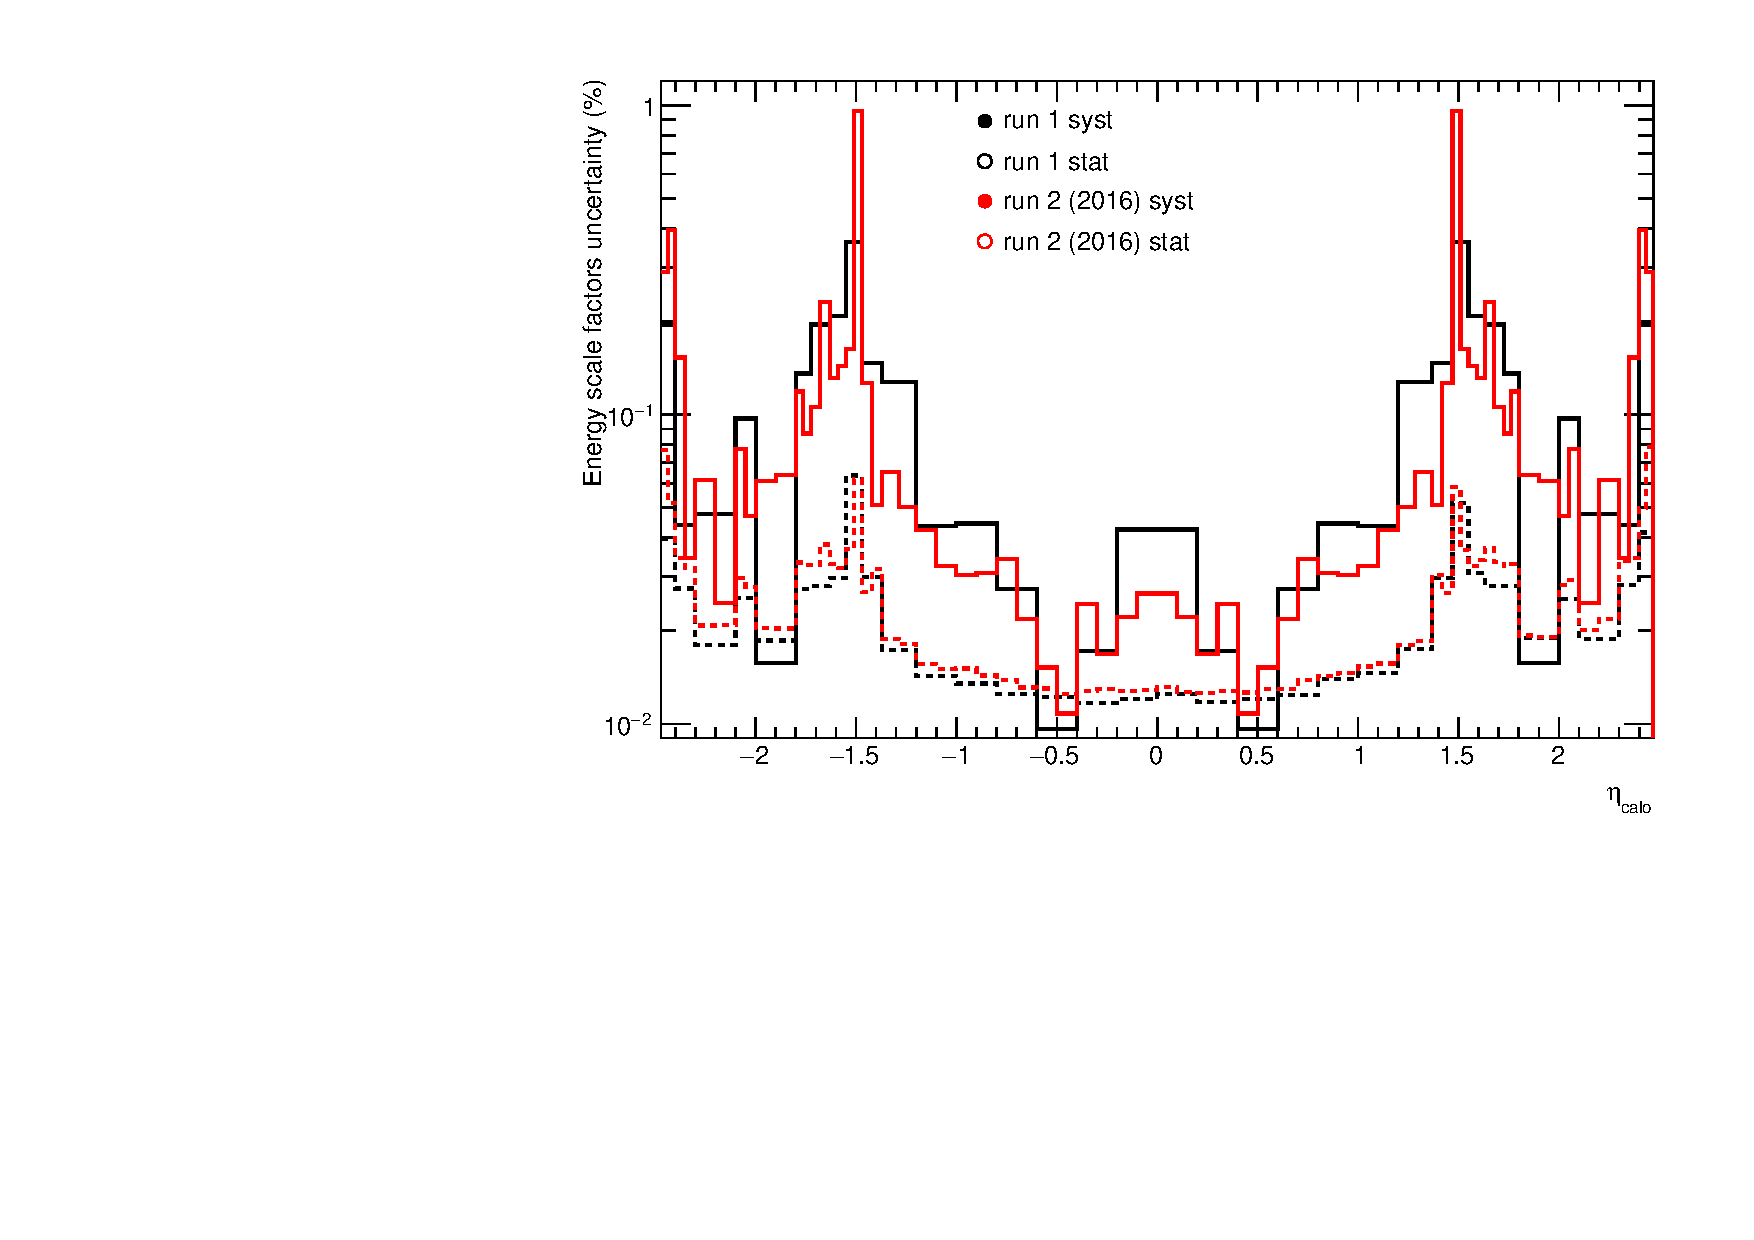
\includegraphics[width=\linewidth]{Figures/CompareSystRun_alpha.pdf}\\
        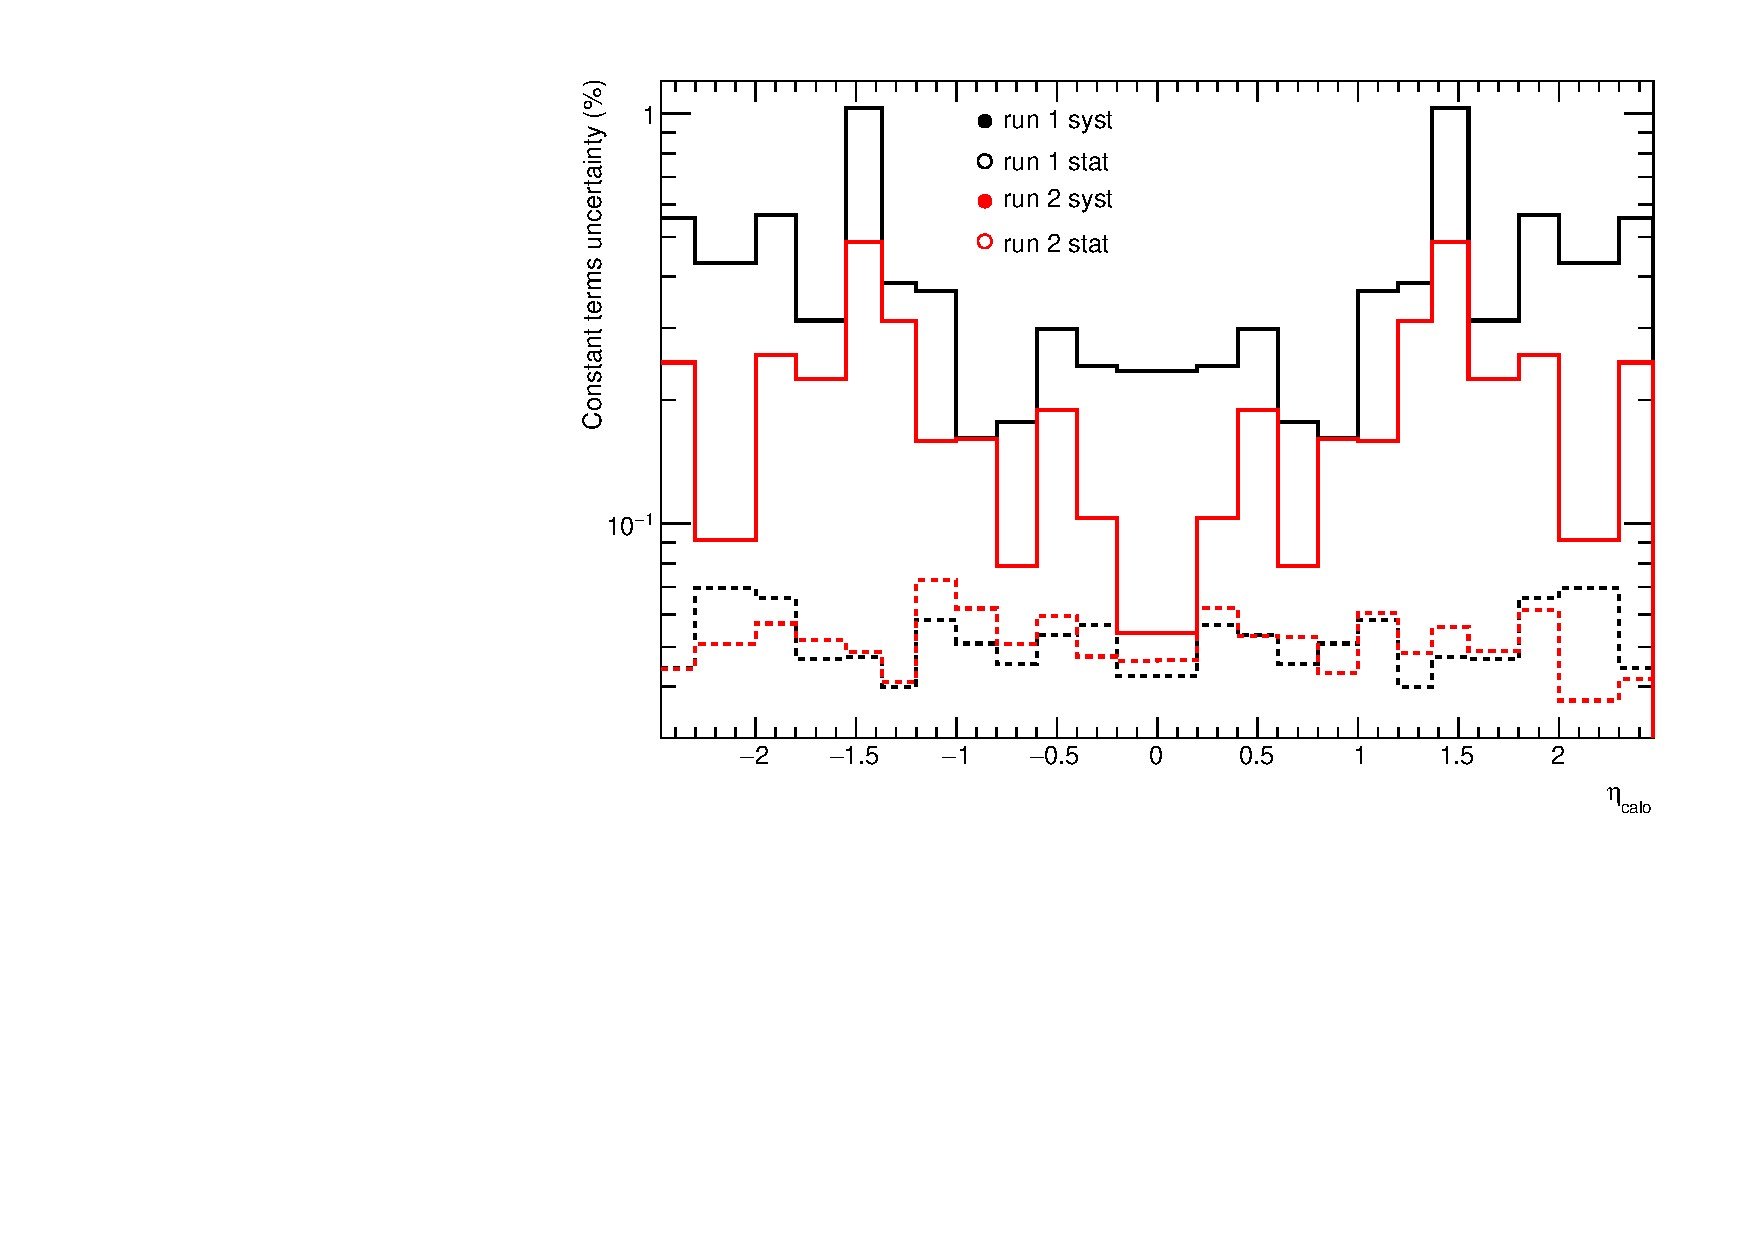
\includegraphics[width=\linewidth]{Figures/CompareSystRun_c.pdf}
  \end{minipage}
  \hfill
  \begin{minipage}{0.54\linewidth}
    \includegraphics[width=\linewidth]{CalibSupNote_Distri_m12_corrected.pdf}
  \end{minipage}

\end{frame}


%===============================================
\section{Measurement of Higgs boson couplings}
\frame{\tableofcontents[currentsection]}

%%=================================================================================
\begin{frame}{Simplified Template Cross Section (STXS) framework}
  \centering
  \includegraphics[width=0.8\linewidth]{HTSX.pdf}\\
  Replace signal strengths ($\mu=\frac{\sigma^{exp}}{\sigma^{th}}$) by cross-section in exclusive phase space regions.
\end{frame}
%%=================================================================================
\begin{frame}{Couplings measurement strategy}

  \begin{minipage}{0.49\linewidth}
  {\bf Inclusive selection }
  \begin{itemize}
  \item 2 tight photons
  \item $\frac{p_T^\gamma}{m_{\gamma\gamma}}>0.35 (0.25)$
  \item $|\eta|\in [0, 1.37]  \cup [1.52, 2.37]$
  \item $m_{\gamma\gamma} \in [105, 160]$ GeV
  \end{itemize}
  \end{minipage}
  \hfill
  \begin{minipage}{0.49\linewidth}
    {\bf Dataset properties}  

    \begin{itemize}
    \item $\sim$ 330k events
    \item $42\%$ signal efficiency
    \item $\simeq 1730$ expected signal yield
    \end{itemize}
  \end{minipage}
  \vfill
  {\bf Analysis strategy } 
  \begin{itemize}
  \item Define reconstructed categories targetting specific truth bin.
  \item Measure acceptance of each category wrt truth bins.
  \item Evaluate systematics effects on signal model.
  \item Combined fit of $m_{\gamma\gamma}$ distribution with signal+bkg model.
  \end{itemize}

\end{frame}

%%=================================================================================
\begin{frame}{Reconstructed categories}
  \begin{minipage}{0.49\linewidth}
      \includegraphics[width=\linewidth]{ATL-COM-PHYS-2016-1784_flowchart-eps-converted-to.pdf}
  \end{minipage}
  \hfill
  \begin{minipage}{0.49\linewidth}
    Optimised sensitivity to :
    \begin{itemize}
    \item rare processes
    \item truth bins
    \item detector resolution
    \end{itemize}
%    \includegraphics[width=\linewidth]{ATLAS-CONF-2017-045_4t.pdf}
  \end{minipage}
\end{frame}

%%=================================================================================
\begin{frame}{Truth bin distribution}
  \begin{minipage}{0.6\linewidth}
      \includegraphics[width=\linewidth]{ATL-COM_PHYS_2016-1784_purity_2D.pdf}
  \end{minipage}
  \hfill
  \begin{minipage}{0.39\linewidth}
    \begin{itemize}
    \item \textcolor{blue}{Columns : distribution of events of a given category over the truth bins.}
    \item Rectangles : process optimised categories
    \end{itemize}
  \end{minipage}
  
  \centering
  \textcolor{red}{\bf Good performances of process targetting}
\end{frame}
%%=================================================================================
\begin{frame}{Calibration uncertainties methodology}

      For each systematic sources (energy scale for example) and each category : 
      \begin{itemize}
      \item Create distributions of :
        \begin{itemize}
        \item $m^\text{nom} = m^{rec}\sqrt{(1+\alpha_1)(1+\alpha_2)}$
        \item \textcolor{red}{$m^\text{up} = m^{rec}\sqrt{(1+\alpha_1 + \Delta\alpha_1)(1+\alpha_2+\Delta\alpha_2)}$}
        \item \textcolor{green}{$m^\text{down} = m^{rec}\sqrt{(1+\alpha_1 - \Delta\alpha_1)(1+\alpha_2-\Delta\alpha_2)} $}
        \end{itemize}

      \end{itemize}

  \begin{minipage}{0.49\linewidth}
    \begin{itemize}
            \item Fit distributions using signal model (Double Sided Crystal Ball)
    \item Define systematic variation : \\$\Delta X = \frac{X^{fluct}}{X^{nom}}-1$ \\ $X\in {\text{mean, RMS, yield}}$
    \end{itemize}
    \end{minipage}
    \hfill
    \begin{minipage}{0.49\linewidth}
      \includegraphics[width=\linewidth]{Figures/h013_EG_SCALE_ALL_0.pdf}
    \end{minipage}

    \vfill
\end{frame}

%=================================================================================
\begin{frame}{Correlation models }
  \begin{center}{\bf Two correlation models : } \end{center}
  \begin{minipage}[t]{0.49\linewidth}
    {\bf 1NP }
    \begin{itemize}
    \item 2NP (scale + resolution)
    \item Fully correlated
    \item Conservative
    \item Faster
    \end{itemize}
  \end{minipage}
  \hfill
  \begin{minipage}[t]{0.49\linewidth}
    {\bf FULL}
    \begin{itemize}
    \item 86 NP (77 scale + 9 resolution)
    \item True correlation
    \end{itemize}
  \end{minipage}
  
  \begin{minipage}{0.49\linewidth}
    \resizebox{\linewidth}{!}{
      \begin{tabular}{l|ll}
        Total Scale Uncertainty (\%) & 1NP & FULL \\
        \hline
        Measurement with $H\rightarrow\gamma\gamma$ MC & 0.46 & 0.27\\
        Formula & 0.47 & 0.26\\
      \end{tabular}
    }
  \end{minipage}
  \hfill
  \begin{minipage}{0.49\linewidth}
    \includegraphics[width=\linewidth]{CompareFULLMerge_mean_InclusiveUp.pdf}
  \end{minipage}

\end{frame}
%=================================================================================
\begin{frame}{Calibration uncertainties results}

  \begin{minipage}{0.49\linewidth}
    \centering
    {\bf 49 Nuisance Parameters }
    \begin{itemize}
    \item 9 for resolution
    \item 40 for scale
    \end{itemize}
    \vfill
    {\bf affecting }
    \begin{itemize}
    \item resolution
    \item mass
    \item yield per category
      \end{itemize}
  \end{minipage}
  \hfill
  \begin{minipage}{0.49\linewidth}
    \begin{tikzpicture}
      \node[anchor=south west] {    \includegraphics[width=\linewidth]{Figures/h015d_FULLMerge_catMerge_Systematics_Inclusive_mean_mean.pdf}};
      \node[draw] at (2.2,3.88) {mean};
    \end{tikzpicture}
  \end{minipage}

  \begin{minipage}{0.49\linewidth}
    \begin{tikzpicture}
      \node[anchor=south west] {    \includegraphics[width=\linewidth]{Figures/h015d_FULLMerge_catMerge_Systematics_Inclusive_sigma_sigma.pdf}};
      \node[draw] at (2.2,3.82) {RMS};
    \end{tikzpicture}
  \end{minipage}
  \hfill
  \begin{minipage}{0.49\linewidth}
    \begin{tikzpicture}
      \node[anchor=south west] {    \includegraphics[width=\linewidth]{Figures/h015d_FULLMerge_catMerge_Systematics_Inclusive_yield_yield.pdf}};
      \node[draw] at (2.2, 3.8) {yield};
    \end{tikzpicture}
  \end{minipage}

\end{frame}
%%=================================================================================
\begin{frame}{Total uncertainty}
  \centering
  Total calibration uncertainty as a function of reconstructed category.\\
\includegraphics[width=0.9\linewidth]{Figures/h015d_FULLMerge_catMerge_Systematics_InclusiveUp.pdf}  
\end{frame}
%%=================================================================================

\begin{frame}{Run 2 $H\rightarrow \gamma\gamma$  couplings results}
  \centering
  Due to lack of statistics, some truth bins have been merged.
  Grey area represents theory uncertainty (not included in measurement).

  \includegraphics[width=0.55\linewidth]{ATLAS-CONF-2017-045_15f.pdf}
%%   \tiny 
%%   \begin{align*}
%%     \sigma (ggH, \mathrm{0~jet}) \tbfhyy &= 63\ ^{+17}_{-16}\ \fb  &= 63\ ^{+15}_{-15}\,\mathrm{(stat.)}\ ^{+8}_{-6}\,\mathrm{(syst.)}\ \fb \\
%%     \sigma (ggH, \mathrm{1~jet}, p_T^{H} < 60\ \text{GeV}) \tbfhyy &= 15\ ^{+13}_{-12}\ \fb  &= 15\ ^{+12}_{-12}\,\mathrm{(stat.)}\ ^{+6}_{-4}\,\mathrm{(syst.)}\ \fb \\
%%     \sigma (ggH, \mathrm{1~jet}, 60 \leq p_T^{H} < 120\ \text{GeV}) \tbfhyy &= 10\ ^{+7}_{-6}\ \fb  &= 10\ ^{+6}_{-6}\,\mathrm{(stat.)}\ ^{+2}_{-1}\,\mathrm{(syst.)}\ \fb \\
%%     \sigma (ggH, \mathrm{1~jet}, 120 \leq p_T^{H} < 200\ \text{GeV}) \tbfhyy &= 1.7\ ^{+1.7}_{-1.6}\ \fb  & = 1.7\ ^{+1.6}_{-1.6}\,\mathrm{(stat.)}\ ^{+0.6}_{-0.4}\,\mathrm{(syst.)}\ \fb \\
%%     \sigma (ggH, \geq 2~\mathrm{jet}) \tbfhyy &= 11\ ^{+8}_{-8}\ \fb  &= 11\ ^{+8}_{-8}\,\mathrm{(stat.)}\ ^{+3}_{-2}\,\mathrm{(syst.)}\ \fb \\
%%     \sigma (qq \rightarrow Hqq, p_T^{j} < 200~\text{GeV}) \tbfhyy &= 10\ ^{+6}_{-5}\ \fb  &= 10\ ^{+5}_{-5}\,\mathrm{(stat.)}\ ^{+2}_{-1}\,\mathrm{(syst.)}\ \fb \\
%%     \sigma (ggH + qq \rightarrow Hqq, \mathrm{BSM-like}) \tbfhyy &= 1.8\ ^{+1.4}_{-1.4}\ \fb  &= 1.8\ ^{+1.3}_{-1.3}\,\mathrm{(stat.)}\ ^{+0.5}_{-0.5}\,\mathrm{(syst.)}\ \fb \\
%%     \sigma (\mathrm{VH, leptonic}) \tbfhyy &= 1.4\ ^{+1.4}_{-1.2}\ \fb  &= 1.4\ ^{+1.3}_{-1.2}\,\mathrm{(stat.)}\ ^{+0.3}_{-0.3}\,\mathrm{(syst.)}\ \fb \\
%%     \sigma (\mathrm{top}) \tbfhyy &= 1.3\ ^{+0.9}_{-0.8}\ \fb  &= 1.3\ ^{+0.9}_{-0.8}\,\mathrm{(stat.)}\ ^{+0.3}_{-0.1}\,\mathrm{(syst.)}\ \fb \\
%% \end{align*}

\end{frame}
%%====================================================================
\begin{frame}{Run 2 $H\rightarrow \gamma\gamma$ signal strength results}
  STXS difficult to interpret directly.\\
  Measurement of signal strengths $\mu_i = \frac{\sigma_i^{exp}}{\sigma_i^{SM}}$  performed ($\mu=1=\text{SM}$).\\

  \begin{minipage}{0.49\linewidth}
    \includegraphics[width=\linewidth]{ATLAS-CONF-2017-045_11f.pdf}
  \end{minipage}
  \hfill
  \begin{minipage}{0.49\linewidth}
    \centering
    \includegraphics[width=0.7\linewidth]{ATLAS-CONF-2017-045_6t.pdf}
  \end{minipage}

  \begin{center}
  \begin{minipage}{0.62\linewidth}
    \begin{itemize}
    \item Major theory improvement wrt run 1
    \item Major resolution improvement wrt run 1
    \item Increase of mass scale impact
    \item   \textcolor{red}{\bf No deviation from SM}
      \end{itemize}
  \end{minipage}

  \end{center}
\end{frame}

%%=============================
\begin{frame}{Conclusion}

  \begin{itemize}
  \item Outstanding LHC performance $\rightarrow$ large statistics available
  \item Major improvement of calibration uncertainties \\
    \textcolor{red}{\bf resolution uncertainties no longer dominant on $\mu$}
  \item Couplings measurement performed with $36.1$~fb$^{-1}$ at $\sqrt{s}=13$~TeV
  \item \textcolor{blue}{\bf No significant deviation from standard model}
    \end{itemize}

  \begin{minipage}{0.39\linewidth}
    \begin{itemize}
    \item Much more data expected until end of run 2
    \item \textcolor{red}{\bf Work on experimental systematics required}
    \end{itemize}
  \end{minipage}
  \begin{minipage}{0.6\linewidth}
    \includegraphics[width=\linewidth]{ATLAS-CONF-2017-045_11f.pdf}
  \end{minipage}
\end{frame}

\begin{frame}
\maketitle
\end{frame}
%% ###################################################################################
%%###################################################################################
%%###################################################################################
\appendix
\section{Experimental context}

%=======================================================
\begin{frame}{OFC : sampling effect}
  \centering
  \begin{figure}[htbp]
    \includegraphics[width=0.8\linewidth]{/home/goudet/Documents/LAL/Zim/Calibration/Data15_13TeV/deltaE_E_OFC.png}
    \caption{\label{fig:org3364702}
      Comparison on 2012 $Z\rightarrow ee$ data of reconstructed energy between 4 and 5 signal samplings.}
  \end{figure}
\end{frame}

%=======================================================
\begin{frame}{Identification variables}
  \begin{center}
\includegraphics[width=0.45\linewidth]{CONF-2014-032_1t.pdf}
\end{center}
\end{frame}

%=======================================================
\begin{frame}{Reconstruction \& Identification efficiencies}
  Not all electrons pass the reconstruction and identification criteria. \\
  {\bf 3 menus with increasing purity ( but deceasing efficiencies) are defined : loose, medium, tight}.
  The efficiency of these procedures is given as a function of the $p_T$ and $\eta$.\\
\begin{minipage}{0.49\linewidth}
  \includegraphics[width=\linewidth]{CONF-2014-032_30fa.pdf}
\end{minipage}
\begin{minipage}{0.49\linewidth}
  \includegraphics[width=\linewidth]{CONF-2014-032_30fb.pdf}
\end{minipage}
\end{frame}

%=======================================================

\begin{frame}{Calibration in-situ : run 1  results and uncertainties}
\begin{minipage}{0.64\linewidth}
  Uncertainties are evaluated as the difference between official scales and the ones measured with a changed parameter. 
  They include :
  \begin{itemize}
  \item electron identification quality from medium to tight.
  \item Z mass window 
  \item electron $p_T$ cut
  \item uncertainties on efficiencies scale factors
  \item energy loss through bremshtrahlung
  \item background
  \item pile-up
  \item measurement method
  \end{itemize}
\end{minipage}
\begin{minipage}{0.35\linewidth}
    \includegraphics[width=\linewidth]{CERN-PH-EP-2014-153_26f.pdf}\\
    \includegraphics[width=\linewidth]{CERN-PH-EP-2014-153_27f.pdf}
\end{minipage}
\end{frame}

\begin{frame}{Calibration MVA variables}
  \begin{itemize}
  \item E\(_{\text{acc}}\) : sum of uncalibrated energies measured in the accordion.
  \item E\(_{\text{0}}\)/E\(_{\text{acc}}\) : ratio of the energy in the presampler over the energy in the accordion.
  \item $E_1/E_2$ : ratio of the uncalibrated energy in the first over the second layer ($E_1/E_2$).
  \item \(\eta_{\text{cluster}}\) :  pseudo rapidity in the ATLAS frame.
  \item Cell index : an integer number defined as the integer part of the division ( \(\eta_{\text{calo}}\)/\(\Delta \eta\)) where \(\eta_{\text{calo}}\) is the cluster pseudo rapidity in the calorimeter frame with \(\Delta \eta\) as the size of one cell in the middle layer. 
  \item $\eta$ position of the cluster with respect to the cell edge.
  \item $\phi$ with respect to the lead absorber. This variable is sensitive to the modulation of the thickness of the absorber as a function of $\phi$.
  \end{itemize}
\end{frame}

%====================================
\begin{frame}{In situ calibration $\eta_\text{calo}$ bin frontiers}
        {\tiny \textcolor{brown}{0} 0.1 \textcolor{brown}{0.2} 0.3 \textcolor{brown}{0.4} 0.5 \textcolor{brown}{0.6} 0.7 \textcolor{brown}{0.8} 0.9 \textcolor{brown}{1} 1.1 \textcolor{brown}{1.2} 1.285 \textcolor{brown}{1.37} 1.42 1.47 1.51 \textcolor{brown}{1.55} 1.59 1.63 1.6775 1.725 1.7625 \textcolor{brown}{1.8} 1.9 \textcolor{brown}{2} 2.05 2.1 2.2 \textcolor{brown}{2.3} 2.35 2.4 2.435 \textcolor{brown}{2.47}}
\end{frame}

%===============================================
\begin{frame}{In-situ 2015 pre-recommandations : binning uncertainty}
  \centering
  \includegraphics[width=0.9\linewidth]{/home/goudet/Documents/LAL/Zim/Calibration/PreRec/150727_ComparisonBins_alpha.png}
  \end{frame}
%===============================================
\begin{frame}{In situ scale uncertainties uncertainties}
  12 (13) sources of uncertainties have been evaluated for $\alpha$ ($c$).

    \begin{minipage}{0.49\linewidth} 
      \includegraphics[width=\linewidth]{CalibSupNote_totUncAlpha.pdf}
  \end{minipage}
  \hfill
  \begin{minipage}{0.49\linewidth}
    \includegraphics[width=\linewidth]{CalibSupNote_totUncC.pdf}
  \end{minipage}

\end{frame}

%===========================================
\begin{frame}{Photon correction}
Electrons scale factors are also applied to photons. 
A residual scale factor ($\Delta\alpha$) is measured from $Z\rightarrow ll\gamma$.

No significant deviation observed.
\newline
  \begin{minipage}{0.49\linewidth}
    \includegraphics[width=\linewidth]{CERN-PH-EP-2014-153_34fa.pdf}
  \end{minipage}
  \hfill
  \begin{minipage}{0.49\linewidth}
    \includegraphics[width=\linewidth]{CERN-PH-EP-2014-153_34fb.pdf}
  \end{minipage}
\end{frame}

%============================================

\begin{frame}{ATLAS run 1 H boson mass measurement}
\centering
$$m_H = 125.36 \pm 0.37 \text{(stat)} \pm 0.18 \text{(syst)}$$
\begin{minipage}{0.49\linewidth}
  \includegraphics[width=\linewidth]{1406_3827_8f.pdf}
\end{minipage}
\hfill
\begin{minipage}{0.49\linewidth}
  \begin{tikzpicture}
    \node[anchor=south west] { \includegraphics[width=\linewidth]{1406_3827_4t.pdf} };
    \draw[step=1.0,black,thin] (0,0) grid (10,4);
    \draw[red, line width=0.5mm, rounded corners =2pt] ( 0.1, 1.05 ) rectangle ( 6.1, 1.35 ) ;
  \end{tikzpicture}
\end{minipage}
    {\bf Statistical uncertainties highly dominant.}\\
    \begin{center}   Run 2 will increase sensitivity to systematics.\end{center}
\end{frame}

%%========================================
\begin{frame}{$\mu_{\gamma\gamma}$ measurement}
%$\mu_{\gamma\gamma}$ is a main variable to measure. It is related to the cross section (production probability) :
$$\mu_{\gamma\gamma}=\frac{(\sigma\times BR)^{meas}}{(\sigma\times BR)^{SM}}=1.17 \pm 0.23 \text{(stat)}\ ^{+0.10}_{-0.08}\text{(syst)}\ ^{+0.12}_{-0.08} \text{(theory)}$$
  \begin{minipage}{0.49\linewidth}
    \includegraphics[width=\linewidth]{1408_7084_19f.pdf}
  \end{minipage}
  \hfill
  \begin{minipage}{0.49\linewidth}
    \begin{tikzpicture}
      \node[anchor=south west] { \includegraphics[width=\linewidth]{1408_7084_19t.pdf} };
%      \draw[step=1.0,black,thin] (0,0) grid (10,4);
      \draw[red, line width=1mm, rounded corners =2pt] ( 1, 2.05 ) rectangle ( 13.7, 3.95 ) ;
    \end{tikzpicture}
  \end{minipage}
If no improvements, \textcolor{blue}{\bf calibration uncertainty will be dominant in run 2}.
\end{frame}

%%=================================================================================
\begin{frame}{Scale impact on width}
  \begin{minipage}{0.49\linewidth}\includegraphics[width=\linewidth]{/home/goudet/Documents/LAL/Zim/Hgam/PhotonSystematic/160826_SpreadGauss.pdf}\end{minipage}
  \hfill
  \begin{minipage}{0.49\linewidth}
    1M random numbers generated on a Gaussian$(\mu=125, \sigma=1)$.
    \begin{itemize}
    \item Initial numbers distribution.
    \item \textcolor{red}{Half events multiplied by $1.002$.}
    \item \textcolor{blue}{Remaining  events multiplied by $1.005$.}
    \item \textcolor{magenta}{Combined distribution of \textcolor{red}{red} and \textcolor{blue}{blue}.}
    \end{itemize}
  \end{minipage}
  \vfill
  Mean (m) and RMS (s) of a fitted gaussians are given in the legend.
  Interpretationof the curve in the next slides.
\end{frame}

%%=================================================================================
\begin{frame}{$\mu /\sigma$ scale correlation}
  \begin{minipage}{0.49\linewidth}\includegraphics[width=\linewidth]{/home/goudet/Documents/LAL/Zim/Hgam/PhotonSystematic/160826_SpreadGauss.pdf}\end{minipage}
  \hfill
  \begin{minipage}{0.49\linewidth}
    Lets assume a gaussian distributed energy distribution.
    Applying energy scale correction gives : $$E\rightarrow E(1+a)$$

  \end{minipage}
      Hence the distribution will be changed to  :
      \begin{equation}
      exp( -\frac{(E-\mu)^2}{2\sigma^2}\
      \rightarrow\
      exp( -\frac{(\frac{E}{1+a}-\mu)^2}{2\sigma^2})
      =
      exp( -\frac{(E-\mu(1+a))^2}{2\sigma^2(1+a)^2})
    \end{equation}
      The new distribution is a \textcolor{red}{shifted gaussian with scaled RMS}.\\
      Given the medium shift of EG\_SCALE\_ALL, we expect \textcolor{red}{$^{+0.4}_{-0.4}\%$} change in resolution.
\end{frame}


%%=================================================================================
\begin{frame}{Inhomegenous scale}
  \begin{minipage}{0.49\linewidth}\includegraphics[width=\linewidth]{/home/goudet/Documents/LAL/Zim/Hgam/PhotonSystematic/160826_SpreadGauss.pdf}\end{minipage}
  \hfill
  \begin{minipage}{0.49\linewidth}
    The RMS of two points separated by $d$ is $d/4$.\\
    If $d$ is the difference between two scale factors, $$d\sim 3.10^{-3} \cdot E_\gamma=0.18$$
   $$\frac{\text{RMS}}{\text{Resolution}} = \frac{d/4}{1.5\text{GeV}} = 3\%$$
  \end{minipage}
\vfill
  The inhomogeneity of the scale factors uncertainties \textcolor{red}{changes the width of the distribution at the percent level}.
  This effect will always increase the width.  
  \vfill
  Black and pink distribution show an illustration of this effect.
\end{frame}

%==============================================================================
\begin{frame}{Scale factors interpretation}
  \begin{minipage}{0.49\linewidth}
    Assume the up fluctuation (red) as data and nominal distribution (black) as MC in the template method.
    One has
    $$m_H^{up}=m_H^{nom}(1+\alpha)$$
    Hence
    $$\delta_{m_H}=\alpha$$
    \end{minipage}
  \begin{minipage}{0.49\linewidth}
    \includegraphics[width=\linewidth]{Figures/h013_EG_SCALE_ALL_0.pdf}
  \end{minipage}
  Furthermore :
  $$\sigma_H^{up}=\sigma_H^{nom} \oplus cE$$
  Hence
  $$\delta_{\sigma_H} = \sqrt{1+\frac{c^2E^2}{\sigma_H^2}}-1$$
  One has to be carefull with resolution uncertainty as the template method is weak to measure small differences.
\end{frame}

%%=================================================================================
\begin{frame}{Method comparison}
  4 different fitting methods are compared : fitting in 3 different ranges and template method cross-check within $[122, 128]$GeV.
  Methods compared on h013 simplified model (2NP).
  
  \begin{minipage}{0.42\linewidth}
   % $$m_{\gamma\gamma}\in [105,160]$$
    \includegraphics[width=\linewidth]{Figures/h013_EG_RESOLUTION_ALL_0_105160.pdf}
  \end{minipage}
  \hfill
  \begin{minipage}{0.14\linewidth}
    $\leftarrow [105,160]$
    $\rightarrow [115,135]$
    \end{minipage}
  \hfill
  \begin{minipage}{0.42\linewidth}
    \includegraphics[width=\linewidth]{Figures/h013_EG_RESOLUTION_ALL_0_115135.pdf}
  \end{minipage}
  \begin{minipage}{0.42\linewidth}
    \includegraphics[width=\linewidth]{Figures/h013_EG_RESOLUTION_ALL_0_120130.pdf}
  \end{minipage}
  \hfill
  \begin{minipage}{0.14\linewidth}
    $\leftarrow [120,130]$
    $\rightarrow [122,128]$
  \end{minipage}
    \hfill
  \begin{minipage}{0.42\linewidth}
    \centering
        \includegraphics[width=0.5\linewidth]{Figures/h013_EG_RESOLUTION_ALL__1up_0_scale.pdf}\\
        $c=(0.598\pm 0.009)\%$\\$\rightarrow \delta_{\sigma_H}=(8.82\pm0.25)\%$
  \end{minipage}
\end{frame}

\end{document}

